\documentclass[11pt]{standalone}
\usepackage{amssymb}
\usepackage{amsmath}
\usepackage[no-math]{fontspec}
\usepackage{unicode-math}
\usepackage{libertinus}
\usepackage{pgf,xcolor}
\usepackage{tikz}
\usetikzlibrary{arrows.meta, backgrounds}
\usepackage{pgfplots}
\pgfplotsset{compat=newest}

\definecolor{my_darkgray}{HTML}{484949}
\definecolor{my_lightgray}{HTML}{F3F4F4}
\definecolor{my_darkblue}{HTML}{005A94}
\definecolor{my_lightblue}{HTML}{CCDEE9}
\definecolor{my_yellow}{HTML}{FFEC7F}
\definecolor{my_red}{HTML}{E60000}
\definecolor{my_orange}{HTML}{E87846}

\begin{document}
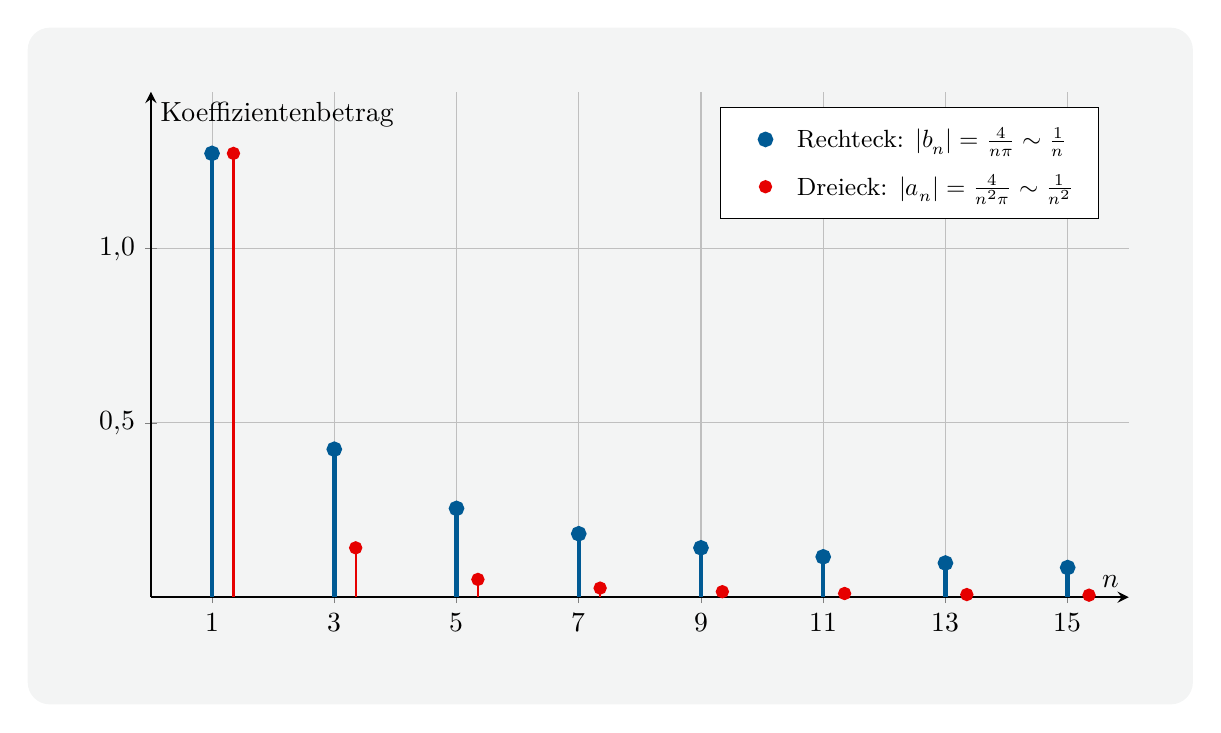
\begin{tikzpicture}[
    show background rectangle,
    background rectangle/.style={fill=my_lightgray, rounded corners=8pt},
    inner frame sep=0.8cm
]
\begin{axis}[
    axis lines = center,
    xlabel = {$n$},
    ylabel = {Koeffizientenbetrag},
    grid = both,
    % axis equal hier bewusst weggelassen: Der Wertebereich der Koeffizienten
    % (bis ca. 1.3) ist viel kleiner als der n-Bereich (bis 15); bei gleicher
    % Skalierung waere das Diagramm unleserlich flach.
    axis line style={thick},
    width=14cm, height=8cm,
    xmin=0, xmax=16,
    ymin=0, ymax=1.45,
    xtick={1, 3, 5, 7, 9, 11, 13, 15},
    ytick={0.5, 1.0},
    yticklabels={$0{,}5$, $1{,}0$},
    legend pos=north east,
    % Die Bruchterme in den Legendeneintraegen sind hoeher als normale
    % Textzeilen; deshalb Zeilenabstand und Innenabstand der Legende erhoehen.
    legend style={font=\small, row sep=4pt, inner xsep=7pt, inner ysep=5pt},
    legend cell align=left,
]
% Rechteck-Lagerkraft (Abschnitt 12.4): |b_n| = 4/(n pi) fuer ungerade n,
% Abklingen wie 1/n
\addplot[ycomb, draw=my_darkblue, ultra thick,
         mark=*, mark options={fill=my_darkblue}]
    coordinates {
    (1, 1.2732)
    (3, 0.4244)
    (5, 0.2546)
    (7, 0.1819)
    (9, 0.1415)
    (11, 0.1157)
    (13, 0.0979)
    (15, 0.0849)
};
\addlegendentry{Rechteck: $|b_n| = \tfrac{4}{n\pi} \sim \tfrac{1}{n}$}
% Dreiecksschwingung (Abschnitt 13.1): |a_n| = 4/(n^2 pi) fuer ungerade n,
% Abklingen wie 1/n^2; leicht versetzt, damit die Staebe nicht ueberlappen
\addplot[ycomb, draw=my_red, thick,
         mark=*, mark options={fill=my_red}]
    coordinates {
    (1.35, 1.2732)
    (3.35, 0.1415)
    (5.35, 0.0509)
    (7.35, 0.0260)
    (9.35, 0.0157)
    (11.35, 0.0105)
    (13.35, 0.0075)
    (15.35, 0.0057)
};
\addlegendentry{Dreieck: $|a_n| = \tfrac{4}{n^2\pi} \sim \tfrac{1}{n^2}$}
\end{axis}
\end{tikzpicture}
\end{document}
